\newpage
\section{Diagrammi di attività}
\subsection{Introduzione}
I diagrammi di attività sono diagrammi che descrivono e modellano un processo. Esso organizza più entità in un insieme di azioni, secondo un determinato flusso.
Il gruppo ha deciso di prendere in esame tre possibili situazioni rilevanti all'interno dell'API Market.

\subsection{Diagramma di attività relativa alla ricerca di una API}
\begin{figure} [H]
	\centering
	\includegraphics[width=1.0\linewidth]{"IMG/ricerca API"}
	\caption{Diagramma di attività che descrive la ricerca di una API}
\end{figure}
\begin{itemize}
	\item \textbf{Precondizioni}: l'utente si trova all'interno dell'API Market e decide di effettuare una ricerca di un'API in base ad alcuni parametri;
	\item \textbf{Postcondizioni}: l'utente ha individuato l'API adatta al suo scopo e potrà acquistarla (vedere diagramma \textit{"Acquisto API"});
	\item \textbf{Descrizione}: l'utente riempie un box di ricerca con i termini desiderati e, in una nuova pagina, visualizza le API corrispondenti ai parametri inseriti. Attualmente, all'utente si presentano due possibili scelte: effettuare una nuova ricerca con parametri diversi, se i risultati della ricerca non soddisfano le sue aspettative, oppure, visualizzare la pagina dedicata ad una API. All'interno di una API si presentano tre possibili scenari: se l'utente è soddisfatto dell'API, può decidere di proseguire l'acquisto, situazione descritta nel diagramma \textit{"Acquisto API"}, oppure ha due alternative, ovvero ritornare ai risultati della ricerca precedente o effettuare una nuova ricerca.
\end{itemize}

\newpage
\subsection{Diagramma di attività relativa all'acquisto di una API}
\begin{figure}[h]
	\centering
	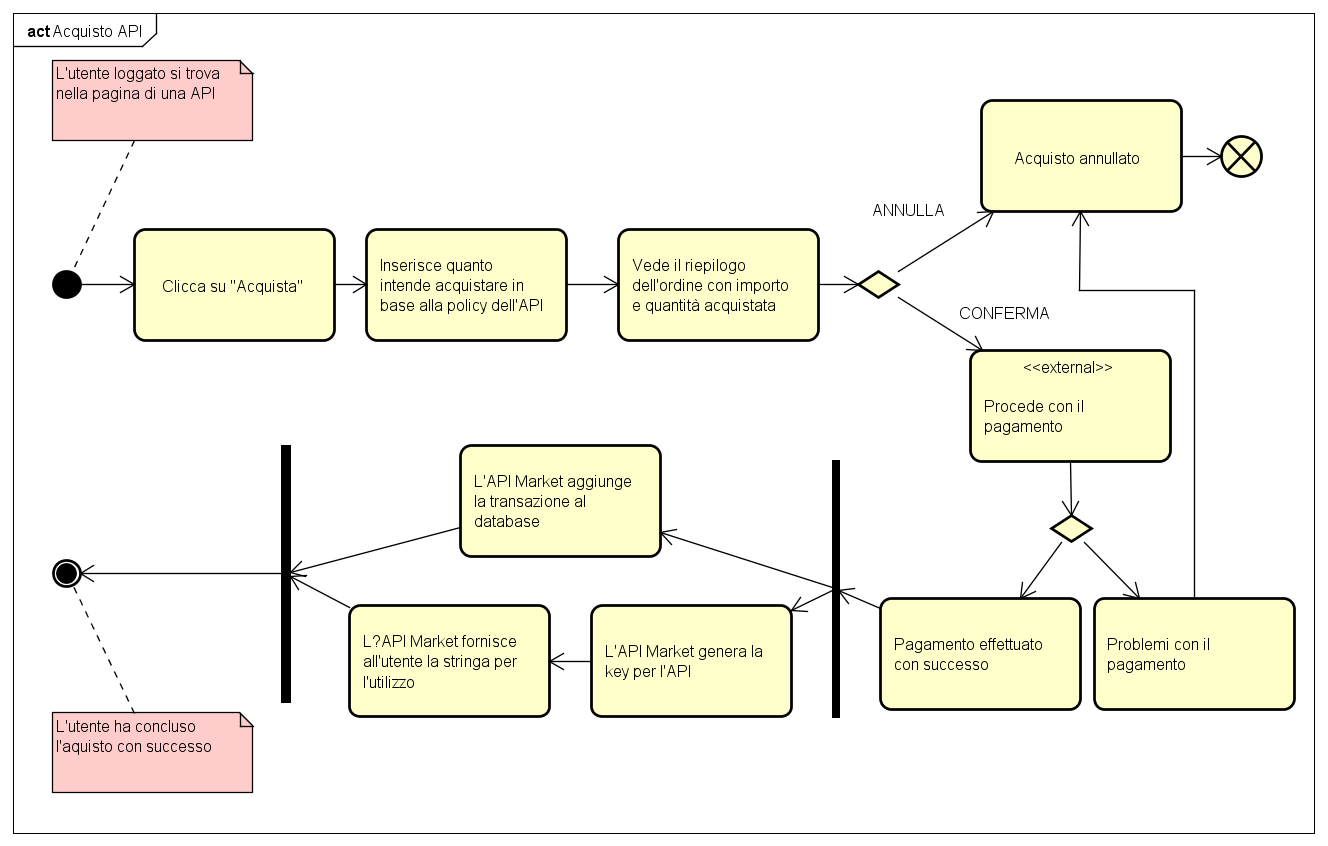
\includegraphics[width=1.0\linewidth]{IMG/Acquisto_API}
	\caption{Diagramma di attività che descrive l'acquisto di un API}
	\label{fig:acquistoapi}
\end{figure}

\begin{itemize}
	\item \textbf{Precondizioni}: l'utente ha scelto un'API dal marketplace e vuole acquistarla;
	\item \textbf{Postcondizioni}: l'utente ha acquistato un'API e può utilizzarla;
	\item \textbf{Descrizione}: inizialmente, l'utente si trova nella pagina dell'API che desidera acquistare. Una volta cliccato su "Acquista", inserisce la quantità che vuole acquistare in base alla policy prevista per quell'API. Successivamente, vedrà un riepilogo dell'acquisto, contenente l'importo in euro e la quantità espressa in base alla policy, ovvero il numero di chiamate, la quantità di traffico espressa in kB oppure il tempo espresso in minuti. L'utente può decidere se confermare il pagamento, tramite la piattaforma PayPal, oppure annullare l'ordine. Il pagamento avviene su un sito esterno ed è possibile che la transazione non vada a buon fine, quindi, è previsto il caso in cui l'utente abbia problemi con il pagamento e l'acquisto venga annullato. Una volta che l'acquisto è confermato, l'API Market aggiungerà la transazione al database, genererà la chiave e fornirà all'utente l'indirizzo e la stringa da utilizzare per chiamare l'API, terminando, di fatto, l'acquisto con successo. 
\end{itemize}

\newpage
\subsection{Diagramma di attività relativa all'inserimento di una API}
\begin{figure}[h]
	\centering
	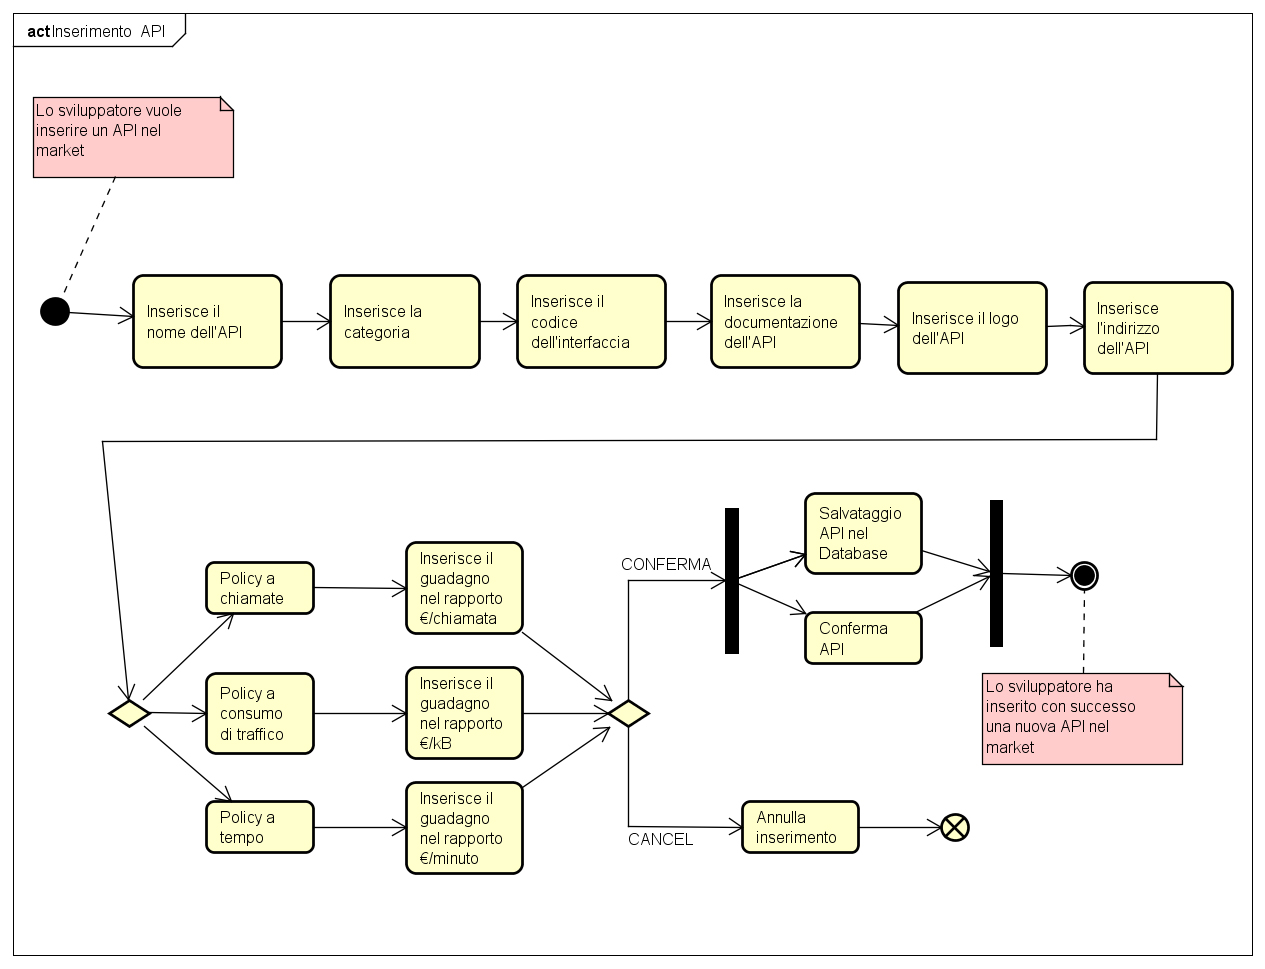
\includegraphics[width=1.0\linewidth]{IMG/Inserimento_API}
	\caption{Diagramma di attività che descrive l'inserimento di un API}
	\label{fig:inserimentoapi}
\end{figure}


\begin{itemize}
	\item \textbf{Precondizioni}: l'utente ha sviluppato un'API e si trova nel proprio profilo, con l'intenzione di pubblicarla sul marketplace;
	\item \textbf{Postcondizioni}: l'utente ha aggiunto un'API al marketplace;
	\item \textbf{Descrizione}: l'utente si trova nel suo profilo e tramite il pulsante "Aggiungi API", carica una sua API sull'API Market. L'utente visualizza, in una nuova pagina, una serie di campi in cui inserire i dati richiesti per la sua API. I dati in questione sono elencati di seguito:
	\begin{itemize}
		\item Nome dell'API;
		\item Categoria di appartenenza dell'API;
		\item Codice dell'interfaccia dell'API;
		\item Documentazione dell'API;
		\item Logo dell'API;
		\item Indirizzo dell'API;
		\item Scelta per la policy e il guadagno della sua API, ovvero:
		\begin{itemize}
			\item \textbf{Policy a chiamate}: definisce il guadagno espresso in euro per ogni chiamata da parte di un acquirente dell'API;
			\item \textbf{Policy a traffico}: definisce il guadagno espresso in euro per ogni kB trasmesso all'acquirente dell'API;
			\item \textbf{Policy a tempo}: definisce il guadagno espresso in euro per ogni minuto di utilizzo da parte di un acquirente dell'API.
		\end{itemize}		
	\end{itemize}
	Successivamente, può decidere se annullare il caricamento oppure confermarlo. Una volta inviata la conferma, l'API Market restituirà una conferma e salverà l'API nel database, rendendola disponibile all'acquisto da parte dei fruitori dell'API Market.
\end{itemize}
